
\newcommand{\printfigGraphTypes}{
    \begin{figure}
        \begin{subfigure}{.5\textwidth}
            \centering
            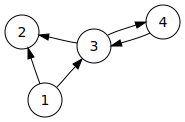
\includegraphics[width=.8\linewidth]{assets/images/Directed_graph_no_background.svg.pdf}
            \caption{Directed graph with cycle between nodes three and four.}
            \label{fig:directedgraph}
        \end{subfigure}
        \begin{subfigure}{.5\textwidth}
            \centering
            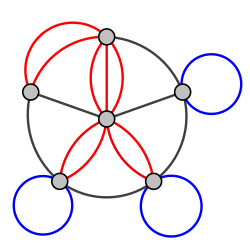
\includegraphics[width=.8\linewidth]{assets/images/Multi-pseudograph.svg.pdf}
            \caption{Multigraph with parallel edges and self-loops}
            \label{fig:multigraph}
        \end{subfigure}%
        \caption[]{Examples of first order graph symantics supported by Jaseci.\footnotemark}
        \label{fig:graph_examples}
    \end{figure}
    \footnotetext{Images credits to wiki contributers~\cite{wiki:Directed_graph_no_background.svg,wiki:Multi-pseudograph.svg}}
}


\newcommand{\printfigHelloWorldBaby}{
    \begin{figure}%{r}{0.5\textwidth}
        \centering
        \includegraphics[width=.3\linewidth]{assets/images/hello_world_baby.jpg}
        \caption[]{World's youngest coder with valid HTML on shirt.\footnotemark}
        \label{fig:hello_baby}
    \end{figure}
    \footnotetext{Image credit to wiki contributer~\cite{wiki:hello_world_baby.jpg}}
}

\newcommand{\printtabPrecedence}{
    \begin{table}[t]
        \footnotesize
        \centering
        \begin{tabular}{l l l}
            \toprule
            \textbf{Rank} & \textbf{Symbol}                            & \textbf{Description}                           \\
            \midrule
            1             & \texttt{( ), [ ], ., ::, spawn}            & Parenthetical/grouping, node/edge manipulation \\
            2             & \texttt{\textasciicircum, []}              & Exponent,  Index                               \\
            3             & \texttt{*, /, \%  }                        & Multiplication, division, modulo               \\
            4             & \texttt{+, -}                              & Addition, subtraction                          \\
            5             & \texttt{==, !=, >=, <=, >, <, in, not in } & Comparison                                     \\
            6             & \texttt{\&\&, ||, and, or  }               & Logical                                        \\
            7             & \texttt{-->, <--, -[]->, <-[]-}            & Connect                                        \\
            8             & \texttt{=, +=, -=, *=, /=, := }            & Assignment                                     \\
            \bottomrule
        \end{tabular}
        \caption{Precedence of operations in Jac}
        \label{tab:jacprecedence} % Unique label used for referencing the table in-text
        %\addcontentsline{toc}{table}{Table \ref{tab:jacprecedence}} % Uncomment to add the table to the table of contents
    \end{table}
}

\newcommand{\printtabStrOps}{
    \begin{table}[t]
        \footnotesize
        \centering
        \rowcolors{1}{light-cyan}{light-gray}
        \begin{tabular}{l p{3cm} p{6cm}}
            \toprule
            \textbf{Op}                                           & \textbf{Args}                                                                                                                                                  & \textbf{Description}                                                                                   \\
            \midrule
            \lstinline{.str::upper}                               & none                                                                                                                                                           &                                                                                                        \\
            \lstinline{.str::lower}                               & none                                                                                                                                                           &                                                                                                        \\
            \lstinline{.str::title}                               & none                                                                                                                                                           &                                                                                                        \\
            \lstinline{.str::capitalize}                          & none                                                                                                                                                           &                                                                                                        \\
            \lstinline{.str::swap\_case}                          & none                                                                                                                                                           &                                                                                                        \\
            \lstinline{.str::is\_alnum}                           & none                                                                                                                                                           &                                                                                                        \\
            \lstinline{.str::is\_digit}                           & none                                                                                                                                                           &                                                                                                        \\
            \lstinline{.str::is\_title}                           & none                                                                                                                                                           &                                                                                                        \\
            \lstinline{.str::is\_upper}                           & none                                                                                                                                                           &                                                                                                        \\
            \lstinline{.str::is\_lower}                           & none                                                                                                                                                           &                                                                                                        \\
            \lstinline{.str::is\_space}                           & none                                                                                                                                                           &                                                                                                        \\
            \lstinline{.str::load\_json}                          & none                                                                                                                                                           &                                                                                                        \\
            \lstinline{.str::count}      & (\textbf{substr}, start, end)            & Returns the number of occurrences of a substring in the given string. Start and end specify range of indices to search                                                                                                                                                  \\
            \lstinline{.str::find}       &   (\textbf{substr}, start, end)            & Returns the index of first occurrence of the substring (if found). If not found, it returns -1. Start and end specify range of indices to search.                                                                                                                       \\
            \lstinline{.str::split}      & \emph{optional} (separator, maxsplit) & Breaks up a string at the specified separator for maxsplit number of times and returns a list of strings. Default separators is ` ' and maxsplit is unlimited.                                                                                                          \\
            \lstinline{.str::join}                                & (params)                                                                                                                                                       & Join elements of the sequence (params) separated by the string separator that calls the join function. \\
            \lstinline{.str::startswith}                          &                                                                                                                                                                &                                                                                                        \\
            \lstinline{.str::endswith}                            &                                                                                                                                                                &                                                                                                        \\
            \lstinline{.str::replace}                             &                                                                                                                                                                &                                                                                                        \\
            \lstinline{.str::strip}                               & optional,                                                                                                                                                      &                                                                                                        \\
            \lstinline{.str::lstrip}                              & optional,                                                                                                                                                      &                                                                                                        \\
            \lstinline{.str::rstrip}                              & optional,                                                                                                                                                      &                                                                                                        \\
            \bottomrule
        \end{tabular}
        \caption{String operations in Jac}
        \label{tab:strops} % Unique label used for referencing the table in-text
        %\addcontentsline{toc}{table}{Table \ref{tab:jacprecedence}} % Uncomment to add the table to the table of contents
    \end{table}
}

\newcommand{\printtabListOps}{
    \begin{table}[t]
        \footnotesize
        \centering
        \begin{tabular}{l l l}
            \toprule
            \textbf{Op}                     & \textbf{Args} & \textbf{Description}               \\
            \midrule
            \lstinline{.list::max}          & none          &                                    \\
            \lstinline{.list::min}          & none          &                                    \\
            \lstinline{.list::idx\_of\_max} & none          &                                    \\
            \lstinline{.list::idx\_of\_min} & none          &                                    \\
            \lstinline{.list::copy}         & none          & Returns a shallow copy of the list \\
            \lstinline{.list::deepcopy}     & none          & Returns a deep copy of the list    \\
            \lstinline{.list::sort}         & none          &                                    \\
            \lstinline{.list::reverse}      & none          &                                    \\
            \lstinline{.list::clear}        & none          &                                    \\
            \lstinline{.list::pop}          & optional,     &                                    \\
            \lstinline{.list::index}        &               &                                    \\
            \lstinline{.list::append}       &               &                                    \\
            \lstinline{.list::extend}       &               &                                    \\
            \lstinline{.list::insert}       &               &                                    \\
            \lstinline{.list::remove}       &               &                                    \\
            \lstinline{.list::count}        &               &                                    \\
            \bottomrule
        \end{tabular}
        \caption{List operations in Jac}
        \label{tab:listops} % Unique label used for referencing the table in-text
        %\addcontentsline{toc}{table}{Table \ref{tab:jacprecedence}} % Uncomment to add the table to the table of contents
    \end{table}
}

\newcommand{\printtabDictOps}{
    \begin{table}[t]
        \footnotesize
        \centering
        \begin{tabular}{l l l}
            \toprule
            \textbf{Op}                 & \textbf{Args} & \textbf{Description}                     \\
            \midrule
            \lstinline{.dict::items}    & (key, default)          & Returns value of key if exists otherwise default                                         \\
            \lstinline{.dict::items}    & none          &                                          \\
            \lstinline{.dict::copy}     & none          & Returns a shallow copy of the dictionary \\
            \lstinline{.dict::deepcopy} & none          & Returns a deep copy of the dictionary    \\
            \lstinline{.dict::keys}     & none          &                                          \\
            \lstinline{.dict::clear}    & none          &                                          \\
            \lstinline{.dict::popitem}  & none          &                                          \\
            \lstinline{.dict::values}   & none          &                                          \\
            \lstinline{.dict::pop}      &               &                                          \\
            \lstinline{.dict::update}   &               &                                          \\
            \bottomrule
        \end{tabular}
        \caption{Dictionary operations in Jac}
        \label{tab:dictops} % Unique label used for referencing the table in-text
        %\addcontentsline{toc}{table}{Table \ref{tab:jacprecedence}} % Uncomment to add the table to the table of contents
    \end{table}
}

\newcommand{\printtabJSAPI}{
    \rowcolors{1}{light-cyan}{light-gray}
    \begin{longtable}{l | p{10cm}}
        \toprule
        \rowcolor{white} \textbf{Interface} & \textbf{Parameters} \\
        \midrule
        \texttt{walker callback} & \texttt{nd: node (*req), wlk: walker (*req), key: str (*req), ctx: dict, \_req\_ctx: dict, global\_sync: bool} \\ \hline
\texttt{walker summon} & \texttt{key: str (*req), wlk: walker (*req), nd: node (*req), ctx: dict, \_req\_ctx: dict, global\_sync: bool} \\ \hline
\texttt{walker register} & \texttt{snt: sentinel, code: str, encoded: bool} \\ \hline
\texttt{walker get} & \texttt{wlk: walker (*req), mode: str, detailed: bool} \\ \hline
\texttt{walker set} & \texttt{wlk: walker (*req), code: str (*req), mode: str} \\ \hline
\texttt{walker list} & \texttt{snt: sentinel, detailed: bool} \\ \hline
\texttt{walker delete} & \texttt{wlk: walker (*req), snt: sentinel} \\ \hline
\texttt{walker spawn create} & \texttt{name: str (*req), snt: sentinel} \\ \hline
\texttt{walker spawn delete} & \texttt{name: str (*req)} \\ \hline
\texttt{walker spawn list} & \texttt{detailed: bool} \\ \hline
\texttt{walker prime} & \texttt{wlk: walker (*req), nd: node, ctx: dict, \_req\_ctx: dict} \\ \hline
\texttt{walker execute} & \texttt{wlk: walker (*req), prime: node, ctx: dict, \_req\_ctx: dict, profiling: bool} \\ \hline
\texttt{walker run} & \texttt{name: str (*req), nd: node, ctx: dict, \_req\_ctx: dict, snt: sentinel, profiling: bool} \\ \hline
\texttt{alias register} & \texttt{name: str (*req), value: str (*req)} \\ \hline
\texttt{alias list} & \texttt{n/a} \\ \hline
\texttt{alias delete} & \texttt{name: str (*req)} \\ \hline
\texttt{alias clear} & \texttt{n/a} \\ \hline
\texttt{global get} & \texttt{name: str (*req)} \\ \hline
\texttt{global set} & \texttt{name: str (*req), value: str (*req)} \\ \hline
\texttt{global delete} & \texttt{name: str (*req)} \\ \hline
\texttt{global sentinel set} & \texttt{snt: sentinel} \\ \hline
\texttt{global sentinel unset} & \texttt{n/a} \\ \hline
\texttt{object get} & \texttt{obj: element (*req), depth: int, detailed: bool} \\ \hline
\texttt{object perms get} & \texttt{obj: element (*req)} \\ \hline
\texttt{object perms set} & \texttt{obj: element (*req), mode: str (*req)} \\ \hline
\texttt{object perms default} & \texttt{mode: str (*req)} \\ \hline
\texttt{object perms grant} & \texttt{obj: element (*req), mast: element (*req), read\_only: bool} \\ \hline
\texttt{object perms revoke} & \texttt{obj: element (*req), mast: element (*req)} \\ \hline
\texttt{graph create} & \texttt{set\_active: bool} \\ \hline
\texttt{graph get} & \texttt{gph: graph, mode: str, detailed: bool} \\ \hline
\texttt{graph list} & \texttt{detailed: bool} \\ \hline
\texttt{graph active set} & \texttt{gph: graph (*req)} \\ \hline
\texttt{graph active unset} & \texttt{n/a} \\ \hline
\texttt{graph active get} & \texttt{detailed: bool} \\ \hline
\texttt{graph delete} & \texttt{gph: graph (*req)} \\ \hline
\texttt{graph node get} & \texttt{nd: node (*req), ctx: list} \\ \hline
\texttt{graph node set} & \texttt{nd: node (*req), ctx: dict (*req), snt: sentinel} \\ \hline
\texttt{graph walk (cli only)} & \texttt{nd: node} \\ \hline
\texttt{sentinel register} & \texttt{name: str, code: str, code\_dir: str, mode: str, encoded: bool, auto\_run: str, auto\_gen\_graph: bool, ctx: dict, set\_active: bool} \\ \hline
\texttt{sentinel pull} & \texttt{set\_active: bool, on\_demand: bool} \\ \hline
\texttt{sentinel get} & \texttt{snt: sentinel, mode: str, detailed: bool} \\ \hline
\texttt{sentinel set} & \texttt{code: str (*req), code\_dir: str, encoded: bool, snt: sentinel, mode: str} \\ \hline
\texttt{sentinel list} & \texttt{detailed: bool} \\ \hline
\texttt{sentinel test} & \texttt{snt: sentinel, detailed: bool} \\ \hline
\texttt{sentinel active set} & \texttt{snt: sentinel (*req)} \\ \hline
\texttt{sentinel active unset} & \texttt{n/a} \\ \hline
\texttt{sentinel active global} & \texttt{detailed: bool} \\ \hline
\texttt{sentinel active get} & \texttt{detailed: bool} \\ \hline
\texttt{sentinel delete} & \texttt{snt: sentinel (*req)} \\ \hline
\texttt{wapi} & \texttt{name: str (*req), nd: node, ctx: dict, \_req\_ctx: dict, snt: sentinel, profiling: bool} \\ \hline
\texttt{architype register} & \texttt{code: str (*req), encoded: bool, snt: sentinel} \\ \hline
\texttt{architype get} & \texttt{arch: architype (*req), mode: str, detailed: bool} \\ \hline
\texttt{architype set} & \texttt{arch: architype (*req), code: str (*req), mode: str} \\ \hline
\texttt{architype list} & \texttt{snt: sentinel, detailed: bool} \\ \hline
\texttt{architype delete} & \texttt{arch: architype (*req), snt: sentinel} \\ \hline
\texttt{master create} & \texttt{name: str (*req), set\_active: bool, other\_fields: dict} \\ \hline
\texttt{master get} & \texttt{name: str (*req), mode: str, detailed: bool} \\ \hline
\texttt{master list} & \texttt{detailed: bool} \\ \hline
\texttt{master active set} & \texttt{name: str (*req)} \\ \hline
\texttt{master active unset} & \texttt{n/a} \\ \hline
\texttt{master active get} & \texttt{detailed: bool} \\ \hline
\texttt{master self} & \texttt{detailed: bool} \\ \hline
\texttt{master delete} & \texttt{name: str (*req)} \\ \hline
\texttt{master createsuper} & \texttt{name: str (*req), set\_active: bool, other\_fields: dict} \\ \hline
\texttt{master allusers} & \texttt{num: int, start\_idx: int} \\ \hline
\texttt{master become} & \texttt{mast: master (*req)} \\ \hline
\texttt{master unbecome} & \texttt{n/a} \\ \hline
\texttt{config get} & \texttt{name: str (*req), do\_check: bool} \\ \hline
\texttt{config set} & \texttt{name: str (*req), value: str (*req), do\_check: bool} \\ \hline
\texttt{config list} & \texttt{n/a} \\ \hline
\texttt{config index} & \texttt{n/a} \\ \hline
\texttt{config exists} & \texttt{name: str (*req)} \\ \hline
\texttt{config delete} & \texttt{name: str (*req), do\_check: bool} \\ \hline
\texttt{logger http connect} & \texttt{host: str (*req), port: int (*req), url: str (*req), log: str} \\ \hline
\texttt{logger http clear} & \texttt{log: str} \\ \hline
\texttt{logger list} & \texttt{n/a} \\ \hline
\texttt{actions load local} & \texttt{file: str (*req)} \\ \hline
\texttt{actions load remote} & \texttt{url: str (*req)} \\ \hline
\texttt{actions load module} & \texttt{mod: str (*req)} \\ \hline
\texttt{actions list} & \texttt{name: str} \\ \hline
\texttt{jac build (cli only)} & \texttt{file: str (*req), out: str} \\ \hline
\texttt{jac test (cli only)} & \texttt{file: str (*req), detailed: bool} \\ \hline
\texttt{jac run (cli only)} & \texttt{file: str (*req), walk: str, ctx: dict, profiling: bool} \\ \hline
\texttt{jac dot (cli only)} & \texttt{file: str (*req), walk: str, ctx: dict, detailed: bool} \\ \hline

        \bottomrule
        \hiderowcolors
        \caption{Full set of core Jaseci APIs}
        \label{tab:jsAPI}
    \end{longtable}
}